\section{Diffusion-Reaction Equation With Nernst Convection Term.}


The complete dynamic system is given by

\begin{align} \label{eq:diffusion-nernst}
\frac{\partial C_+}{\partial t} &= \mathcal{D_+}\left(\nabla^2 C_+(x) +\nabla \cdot \qty{C_+(x)\qty{\frac{z \mathcal{F}}{RT}\nabla\phi(x)}}\right), \\
\frac{\partial C_-}{\partial t} &= \mathcal{D_-}\left(\nabla^2 C_-(x) -\nabla \cdot \qty{C_-(x)\qty{\frac{z \mathcal{F}}{RT}\nabla\phi(x)}}\right),\\
	\nabla^2 \phi &= \frac{\qty{z\mathcal{F}}}{\epsilon}\qty{C_- - C_+}.
\end{align}

Boundary conditions are fixed by the flux at the interface and boundary conditions at the bulk.

\begin{align}
    J_+(x = 0) &= -\mathcal{D}_+\qty{\frac{\partial C_+}{\partial x} - C_+ \frac{z\mathcal{F}}{RT}\frac{\partial\phi}{\partial x}}\bigg|_{x= 0}= -k_f C_+(x = 0, t)\\
    J_-(x = 0) &= -\mathcal{D}_-\qty{\frac{\partial C_-}{\partial x} + C_- \frac{z\mathcal{F}}{RT}\nabla\phi} \bigg|_{x= 0} = 0\\
    C_+(\delta) = C_b\\
    C_-(\delta) = C_b\\
    \phi(x = 0) &= V_0\\
    \phi(x = \delta) &= 0
\end{align}

Initial conditions are given by

\begin{align}
	C_s(x, t=0) = 0,\\
	\phi (x,t=0) = 0.
\end{align}

Let 

\begin{align}
	\Psi(x, t) = \frac{z\mathcal{F}}{RT}\phi(x, t), \\
	\rho_s(x, t) = \frac{C_s(x, t)}{C_b}
\end{align}

be the adimentional potential and adimentional concentration where $s=\pm$ and 

\begin{align}
	\kappa = \sqrt{\frac{\qty{z\mathcal{F}}^2C_b}{\epsilon RT}}.
\end{align}

be the ionic force. Also, we define the adimentional distance parameter $\xi$ and the adimentional time parameter $\tau$ defined as

\begin{align}
	\xi = \kappa x, \\
	\tau = D_+\kappa^2 t
\end{align}

We rewrite equations \ref{eq:diffusion-nernst} as an adimentional system of equations

\begin{align}
\label{eq:adimetional-diffusion-nernst}
    \frac{\partial \rho_+}{\partial \tau} &= \qty{\nabla_\xi^2 \rho_+ - \nabla_\xi\qty{\rho_+ \nabla_\xi \Psi}}, \\
    \frac{\partial \rho_-}{\partial \tau} &= \frac{\mathcal{D}_-}{\mathcal{D_+}}\qty{\nabla_\xi^2 \rho_- + \nabla_\xi\qty{\rho_- \nabla_\xi \Psi}}, \\
    \nabla_\xi^2 \Psi &= \kappa^2\qty{\rho_- - \rho_+}.
\end{align}


In our adimentional units we get

\begin{align}
    J_+(\xi = 0) &= -\mathcal{D}_+\kappa C_+\qty{\frac{\partial \rho_+}{\partial \xi} - \rho_+ \frac{\partial\Psi}{\partial \xi}}\bigg|_{x= 0}= -k_f C_b\rho_s(\xi = 0, \tau)\\
    J_-(\xi = 0) &= -\mathcal{D}_-\kappa C_-\qty{\frac{\partial \rho_-}{\partial \xi} + \rho_- \frac{\partial\Psi}{\partial \xi}}  \bigg|_{x= 0} = 0\\
    \rho_+(\delta) = 1\\
    \rho_-(\delta) = 1\\
    \Psi(\xi = 0) &= \frac{z\mathcal{F}}{RT} V_0 = \Psi_0\\
    \Psi(\xi = \kappa \delta) &= 0
\end{align}

And the adimentional initial conditions are

\begin{align}
	\rho_s(\xi, \tau = 0) = 0,\\
	\Psi (\xi, \tau = 0) = 0.
\end{align}


\subsection{Discrete equations}

In order to obtain the numerical solution of our system, we need to discretize equations \ref{eq:diffusion-nernst}. For each species ($s = \pm$) we have

\begin{align}
    \rho_s^{n+1, k} =& \rho_s^{n,k} \qty{1 - 2 \alpha_s + s \alpha_s \qty{\Psi^{n, k} - \Psi^{n, k-1}}} \\ & + \alpha_s \rho_s^{n, k+1} \qty{1 - s \qty{\Psi^{n,k+1} - \Psi^{n,k}}} + \alpha_s \rho_s^{n,k-1},\\
    \Psi^{n+1, k+1} - 2\Psi^{n+1,k} + \Psi^{n+1, k-1} =& \Delta \xi^2 \qty{C_+^{n+1, k} - C_-^{n+1, k}}.
\end{align}

where we have defined 

\begin{eqnarray*}
	\alpha_+ = \frac{\Delta \tau}{\Delta \xi^2}\\
	\alpha_- = \frac{\Delta \tau}{\Delta \xi^2}\frac{\mathcal{D}_-}{\mathcal{D}_+}.
\end{eqnarray*}
Boundary conditions need to be discretized accordingly

\begin{align}
\rho_s^{n+1, 0} &= \gamma_s \rho_s^{n+1, 1},\\
\rho_s^{n+1, M} &= 1,\\
\Psi^{n+1, 0} &= \Psi_0,\\
\Psi^{n+1, M} &= 0,\\
\Psi^{n+1, M} &= \Psi^{n+1, M-1} .
\end{align}


with

\begin{align}
\gamma_+ &= \frac{1}{1 + \frac{\Delta \xi}{\mathcal{D}_+}\frac{k_f}{\kappa} + \qty{\Psi^{n+1, 1}-\Psi^{n+1,0}} }, \\
\gamma_- &= \frac{1}{1 - \qty{\Psi^{n+1, 1}-\Psi^{n+1,0}} }
\end{align}

This equations yield the following boundary equations

$$ k=1 $$

\begin{align}
    \rho_s^{n+1, 1} = \rho_s^{n,1} \qty{1 - 2 \alpha_s + \alpha_s \gamma_s + s \alpha_s \qty{\Psi^{n, 1} - \Psi^{n, 0}}} + \alpha_s \rho_s^{n, 2} \qty{1 - s \qty{\Psi^{n,2} - \Psi^{n,1}}},\\
    \Psi^{n+1, 2} - 2\Psi^{n+1,1} + \Psi^{n+1, 0} =& \Delta \xi^2\qty{C_+^{n+1, 1} - C_-^{n+1, 1}}.
\end{align}


$$ k = m-1 $$

\begin{align}
    \rho_s^{n+1, m-1} = \rho_s^{n,m-1} \qty{1 - 2 \alpha_s + s \alpha_s \qty{\Psi^{n, m-1} - \Psi^{n, m-2}}} + \alpha_s \rho_s^{n, m} \qty{1 - s \qty{\Psi^{n,m} - \Psi^{n,m-1}}},\\
    \Psi^{n+1, 2} - 2\Psi^{n+1,1} + \Psi^{n+1, 0} = \Delta \xi^2 \qty{C_+^{n+1, 1} - C_-^{n+1, 1}}.  
\end{align}

\subsection{Matrix equations}

We can write the system as follows

\begin{align}
\underline{\rho_s^{n+1}} = (\bf{A} + s\alpha_s\bf{B}(\Psi^{n}) ) \cdot \underline{\rho_s^{n}} + \bf{b_s},\\
\bf{D} \underline{\Psi}^{n+1} = \Delta \xi ^2\qty{\underline{C_-}^{n+1} - \underline{C_+}^{n+1}}- \underline{b}_{\Psi}.
\end{align}


where

\begin{align}
A = \begin{bmatrix}
    1 - 2 \alpha_s + \alpha_s \gamma_s   &  \alpha_s   & 0  &   \cdots & 0   &   0   &   0   &   0 \\
    \alpha_s    &   1 - 2 \alpha_s       &  \alpha_s   & 0  & \cdots   & 0   &   0   &   0 \\
    0         & \alpha_s               &  1 - 2 \alpha_s  & \alpha_s   & \cdots   &   0   &   0   &   0 \\
    \vdots    &  \vdots              &\vdots          &  \vdots  & \vdots   &\vdots & \vdots & \vdots \\ 
    0         &  0                   &  \cdots        &  0       &  \alpha_s    &  1-2\alpha_s &    \alpha_s   &    0 \\
0         &  0                   &  \cdots        &  0           &  0         &     0      &  \alpha_s    &  1-2\alpha_s 
\end{bmatrix},
\end{align}


\begin{align}
B(\Psi) = \begin{bmatrix}
    \qty{\Psi^{n,1} - \Psi^{n, 0}}   &  -\qty{\Psi^{n,2} - \Psi^{n, 1}}   & 0  &   \cdots   0   &   0   &   0 \\
    0                                &  \qty{\Psi^{n,1} - \Psi^{n, 0}}    & -\qty{\Psi^{n,2} - \Psi^{n, 1}}   & 0  & \cdots    &   0 \\
    \vdots    &  \vdots              &\vdots           &\vdots & \vdots & \vdots \\ 
    0         &  0                   &  \cdots        &  0              & \qty{\Psi^{n,M-2} - \Psi^{n, M-3}}   & -\qty{\Psi^{n,M-1} - \Psi^{n, M-2}} \\
0         &  0                   &  \cdots              &     0      &  0    &  \qty{\Psi^{n,M-1} - \Psi^{n, M-2}}
\end{bmatrix}.
\end{align}

Also, 
\begin{align}
D = \begin{bmatrix}
    -2   &  1   & 0  &   \cdots & 0   &   0   &   0   &   0 \\
    1    &  -2    & 1   & 0  & \cdots   & 0   &   0   &   0 \\
    0         & 1                    &  -2   & 1 & \cdots    &   0   &   0 \\
    \vdots    &  \vdots              &\vdots          &  \vdots  & \vdots   &\vdots & \vdots & \vdots \\ 
    0         &  0                   &  \cdots        &  0       &  0         &  0         & -2   & 1 \\
0         &  0                   &  \cdots        &  0           &  0         &     0      &  1    &  -2
\end{bmatrix},
\end{align}

\begin{align}
    b_\Psi = \begin{bmatrix}
        \Psi_0\\
        0\\
        \vdots\\
        0
    \end{bmatrix},
\end{align}

\begin{align}
    b_s = \begin{bmatrix}
        0\\
        0\\
        \vdots\\
        0\\
        1\end{bmatrix}.
\end{align}



\begin{figure}[htbp]
\centering
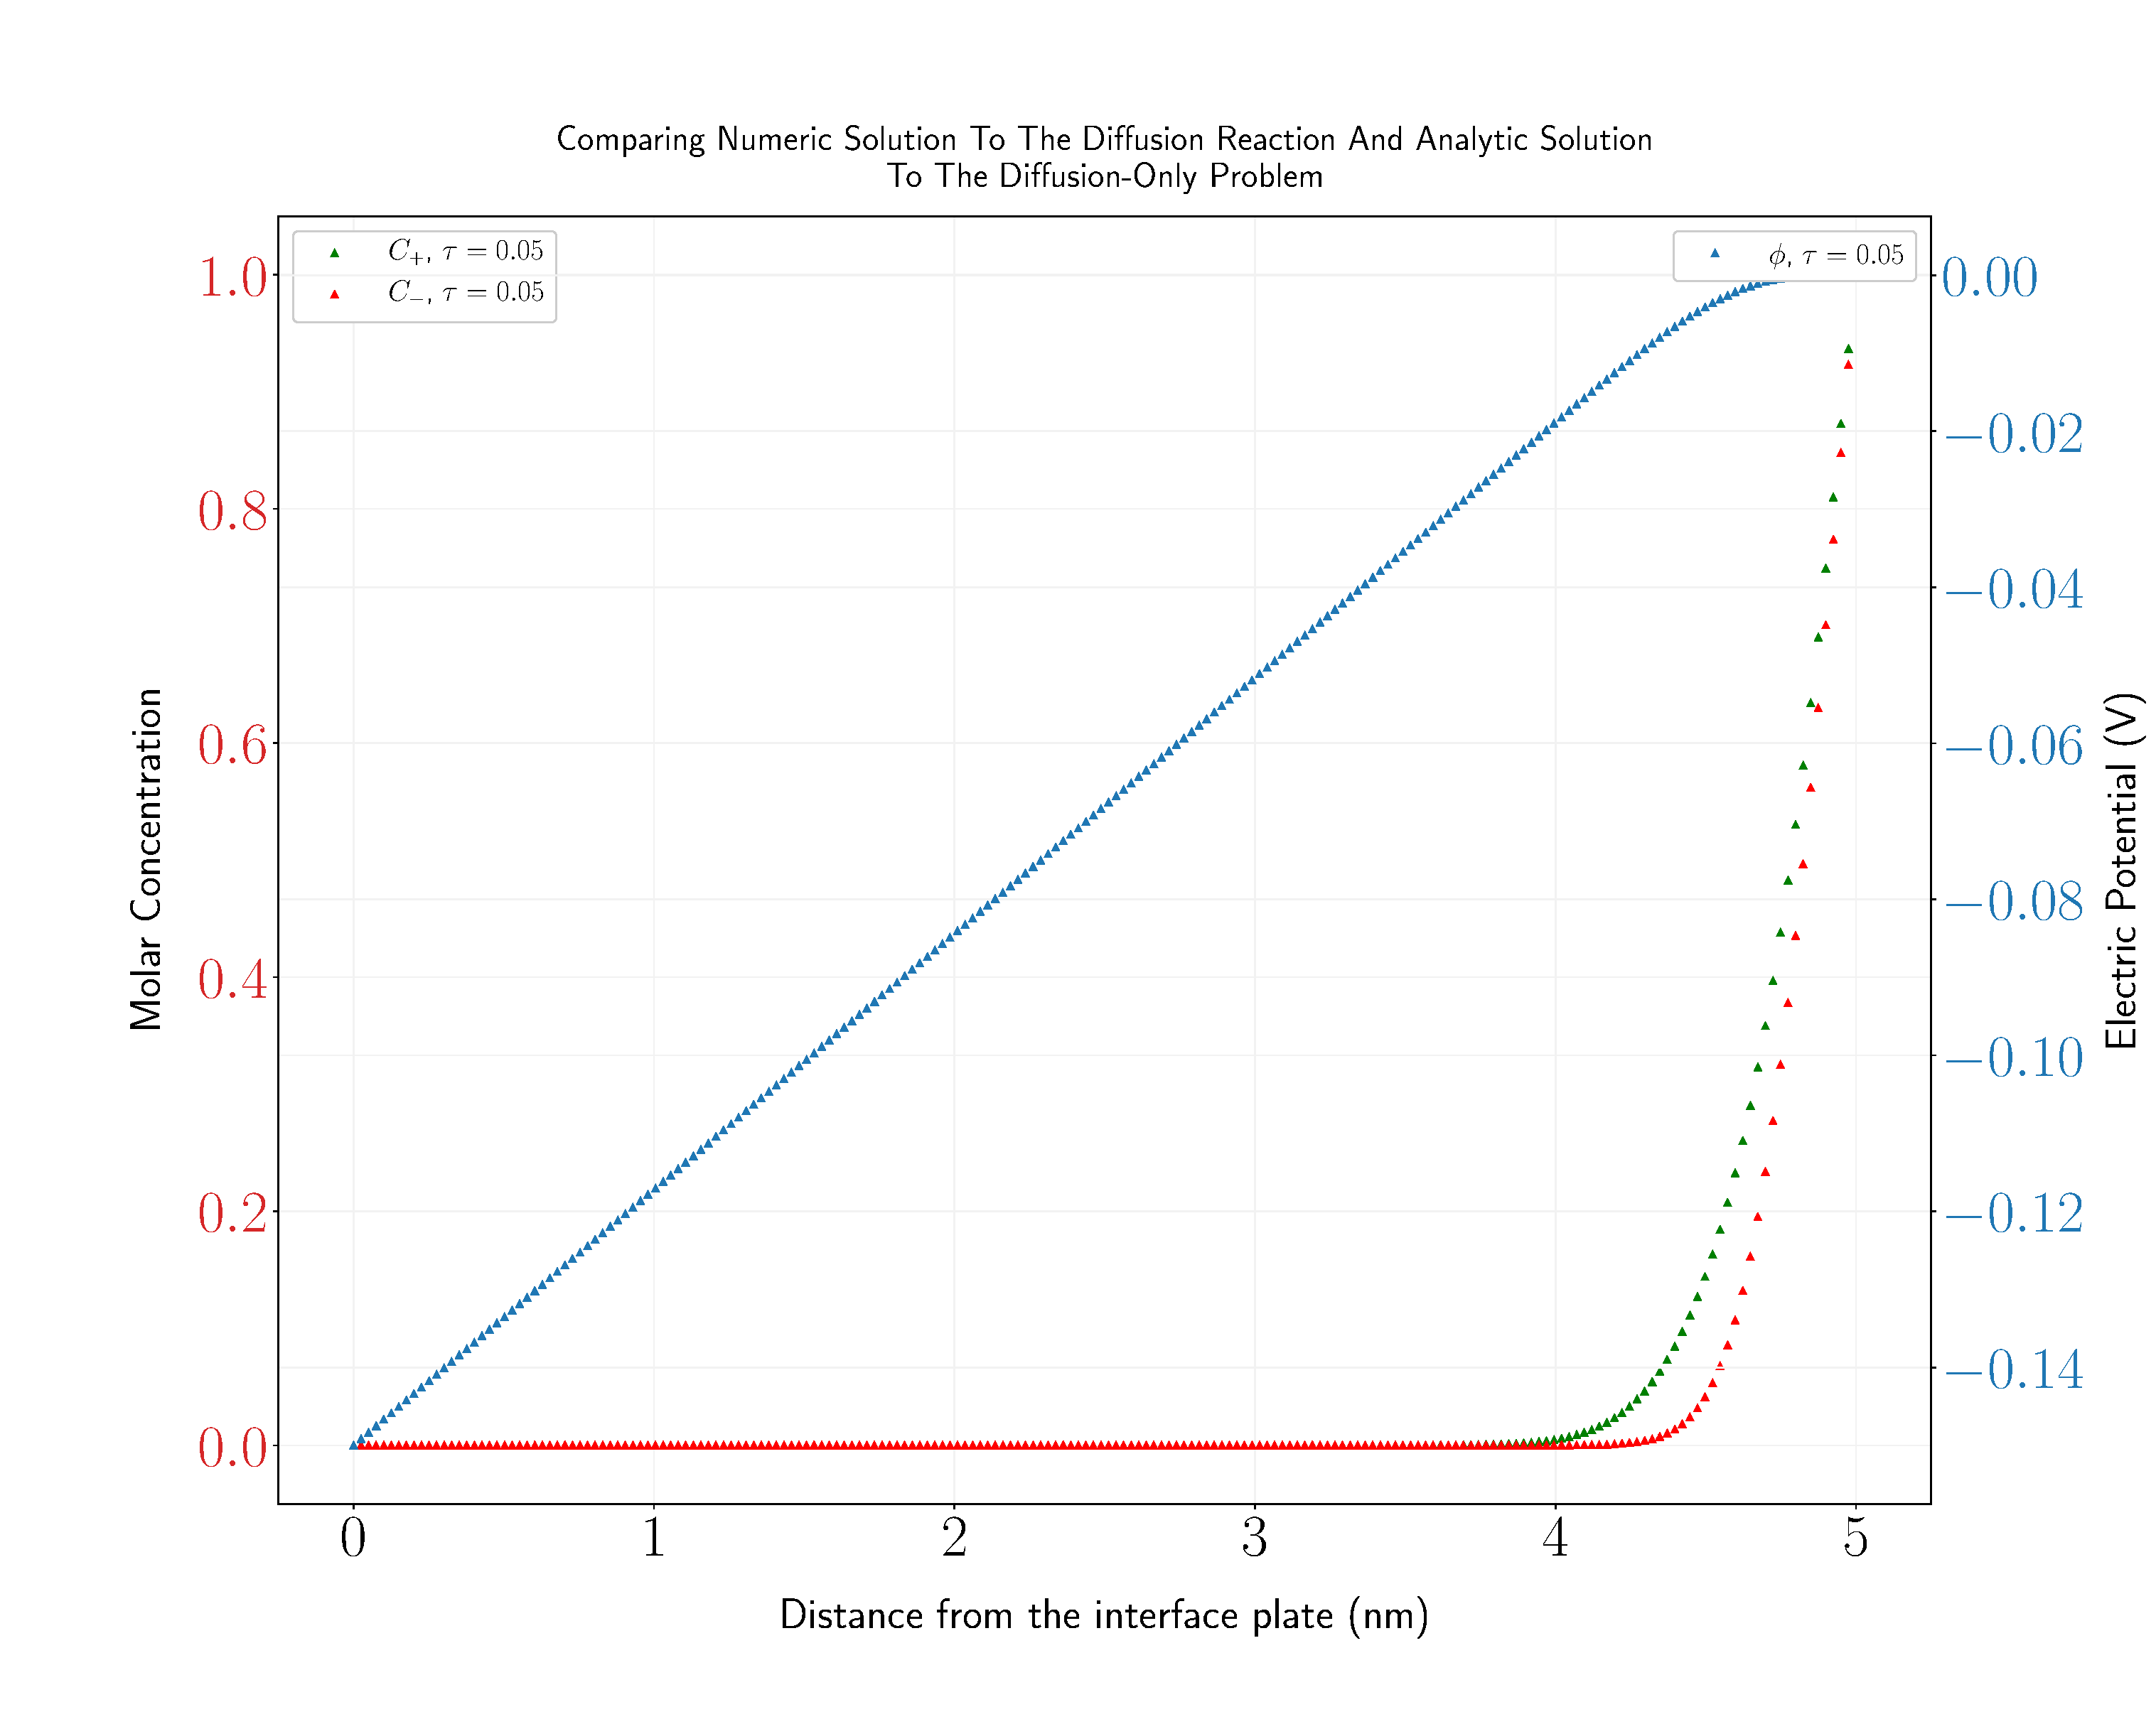
\includegraphics[width=\textwidth]{complete-diffusion-nernst.eps}
\caption{Numerical solution to system \ref{eq:diffusion-nernst}. Red and green dots represent the negative ($SO_4^{-2}$ and positive $Cu^{+2}$ electrolyte concentrations respectively (left axis). The blue dots represent the electric potential (right axis).}
\label{fig:diffusion-comparison}
\end{figure}









